\documentclass[a4paper,11pt]{article}

\usepackage[top=1in, bottom=1.25in, left=1.25in, right=1.25in]{geometry}
\usepackage{graphicx}
\usepackage{amsmath}
\usepackage{amssymb}
\usepackage[style=numeric-comp,sorting=none]{biblatex}
\usepackage{warning} % for warning messages

\parskip=1.5ex
\parindent=0pt

\usepackage{url}
\usepackage{microtype}
\usepackage{lmodern}
\usepackage[colorlinks=true, citecolor=red, linkcolor=blue]{hyperref}

\usepackage{caption}
\usepackage{subcaption}
\usepackage{float}
\usepackage{booktabs}
\usepackage{multirow}
\usepackage[affil-it]{authblk}


\usepackage{todonotes}

\usepackage{siunitx}

\usepackage[compat=1.1.0]{tikz-feynman} % generate feynman diagrams

\renewcommand{\vec}{\mathbf}
\newcommand{\ts}{\textsuperscript}

\bibliography{references}
\overfullrule=2cm % allows to find overfull hboxes much quicker

\binoppenalty=3000
\relpenalty=3000
\clubpenalty=10000
\widowpenalty=10000

\title{Constraining the Standard Model Effective Field Theory with 2D differential cross section of top quark pair production}
\author{Alexander Veltman\\{\small Advisor: Dr.\ James Keaveney}}
\affil{Department of Physics,\\University of Cape Town}

\begin{document}
\maketitle

\begin{abstract}
\end{abstract}
\newpage
\section{Introduction}

The Standard Model (SM) is the best description of nature at the subatomic level that modern physics has to offer.
It describes a collection of particles and the forces between them which are mediated by other particles.
The predictions of physical observables made by the SM can be verified to extreme precision using the latest measurements taken from particle colliders such as the LHC at CERN.
However, there is still some phenomena which are not explained in the SM.
It does not provide an explanation for dark energy and dark matter, for electroweak symmetry breaking or for the Gauge hierarchy problem~\cite{morrissey2012}..
Though the quantity of data available to physicists are orders of magnitudes greater than years prior to the construction of the LHC, no direct searchs for beyond Standard Model (BSM) phenomena have found conclusive evidence of BSM physics at the energies scale of the LHC.

The lack of observations of new physics could be the result of two possible options.
There is the possibility that new physics which may describe the short-comings of the SM exists but is very weakly coupled to the SM particles.
This would make identifying this physics incredibly difficult with the current methods with which particle physics is measured.
The other option suggests that this new physics occurs at energies far larger than what is achieved within the most advanced particle collider, the LHC.
If the SM is considered to be an effective field theory, it is expected that this heavier physics will result in effective interactions which could be identified at the current energy level of the LHC.
This is the motivation of what is known as the Standard Model effective field theory (SMEFT).

SMEFT is a theoretical framework which introduces a set of higher dimensional operators into the SM with a coupling constant for each operator.
These operators describe possible effective interactions induced by heavier physics and are suppressed by the energy scale squared of the new physics.
Due to the increase in detailed measurements of processes such as top pair production, it is possible to use LHC data in order to estimate the couplings for the SMEFT operators.

This report applies the framework of SMEFT to a two sets of top quark observables from the ATLAS experiment at CERN.
This involves a comparison of 1D and 2D differential cross section top pair data in order to determine their ability to constrain top quark related SMEFT operators.
The following report is outlined as follows.
It begins with some contextual information regarding the top physics in section~\ref{sec:topquarks}, an brief overview of the ATLAS detector in section~\ref{sec:ATLAS} and a more detailed explanation of SMEFT in section~\ref{sec:smeft}.
This will lead into section~\ref{sec:deft} in which a description of the SMEFT analysis package dEFT is provided.
The analysis beginning in section~\ref{sec:analysis} will describe the ATLAS data used in the report and will then be proceeded by the details of the Monte Carlo event generation required.
The analysis was performed for both a single top related operator in section~\ref{sec:analysis_one_op} and then using two operators in section~\ref{sec:analysis_two_op}.

\section{Top Physics}\label{sec:topquarks}

The top quark is the most massive particle in the Standard Model with a mass of $m_{t} =172.76\pm0.30$GeV~\cite{ParticleDataGroup:2020ssz} and is commonly used as an area to look for physics beyond the Standard Model.
It participates in both electroweak and strong interactions.

At the LHC, top quarks are usually produced in top-antitop pairs through the $gg\rightarrow t\bar{t}$ and $q\bar{q}\rightarrow t\bar{t}$ processes at leading order.
Leading order (LO) and next-to-leading order (NLO) refer to the number of interactions required for the process to occur.
An example of a LO process is $gg\rightarrow t\bar{t}$ which involves the incoming gluons annihilating into a single gluon which then decays into a top quark pair with no additional particles being created or annihilated.
The Feynman diagrams for these LO processes can be seen in Figure~\ref{fig:ttbar_production}.
It shows that no additional particles other than a single mediating particle and the initial and final states are present in the diagrams.
At the centre of mass energy of the $pp$ collision at the LHC, about 90\% of $t\bar{t}$ production occurs through $gg\rightarrow t\bar{t}$.

\begin{figure}[htb]
    \centering
    \begin{subfigure}[b]{0.4\textwidth}
        \centering
        \feynmandiagram[horizontal=a to b] {
            i1 -- [gluon] a -- [gluon] i2,
            a -- [gluon] b,
            f1 [particle=$\bar{t}$] -- [fermion] b -- [fermion] f2 [particle=$t$],
        };
    \end{subfigure}
    \hfill
    \begin{subfigure}[b]{0.4\textwidth}
        \centering
        \feynmandiagram[horizontal=a to b] {
            i1 [particle=$q$] -- [fermion] a -- [fermion] i2 [particle=$\bar{q}$],
            a -- b,
            f1 [particle=$\bar{t}$] -- [fermion] b -- [fermion] f2 [particle=$t$],
        };
    \end{subfigure}
    \caption{Lowest order Feynman diagrams for top quark pair production through $gg \rightarrow t\bar{t}$ and $q\bar{q} \rightarrow t\bar{t}$.}
    \label{fig:ttbar_production}
\end{figure}

\todo{ask james for sources and context}
Top quarks almost always decays into a $W$ boson and a $b$ quark since the top quark is unable to hadronise.
Due to the $t$ having the largest mass of the quarks, it is actually the only quark which can decay in this manner.
Top quark pair decay is characterised is by the manner in which the two W bosons produced by each of the tops decay.
The tops are then classified as decaying leptonically if the $W$ decays into a lepton and an associated neutrino or hadronically if the $W$ decays into 2 quarks.
Any resulting quarks in the final state hardonise to form jets of hadrons.
Due to high luminosity achieved by the LHC, detailed cross sectional measurements has allowed for the implementation of differential cross section measurements of top quark production into analyses.
This provides differential cross sectional information with respect to the change of an observable as opposed to integrated cross section which is the total cross section.



\nocite{Thomson:2013zua}
The interest in the top quark in terms of beyond standard model physics is due to it being the quark with the largest coupling to the Higgs boson with a Yukawa coupling $y_{t} \approx 1$.
This implies that the top is a major contributor to the first order correction of the Higgs mass which is related to the hierarchy problem.
Deviations of the top coupling or new top interactions are predicted by many BSM theories.
Since the birth of the LHC, the large quantities of top related measurements have allowed for incredible precision which has made the search for this exotic physics possible.

\section{LHC and the ATLAS experiment}\label{sec:ATLAS}
The Large Hadron Collider (LHC) is a two-ring-superconducting particle accelerator located at the European Organization for Nuclear Research (CERN) and is the centre-piece of proton-proton collision physics.
The design consists of two counter-rotating proton beams in a circular ring with a diameter of \SI{26.7}{\kilo\metre}.
During the years of 2016 to 2018, the maximum achievable centre-of-mass energy $\sqrt{s}$ at the LHC was \SI{13}{\tera\electronvolt} with a luminosity of \si{10^{34}\centi\metre\squared\per\second}.
Upgrades have been performed in recent years to allow energies of \SI{14}{\tera\electronvolt}.~\nocite{Evans:2008zzb}
These energies are the highest to be achieved for a particle collider and has allowed for notable landmarks in particle physics including the discovery and verification of the Higgs Boson.
The LHC is home to a family of detector experiments including ATLAS, ALICE, CMS and LHCb.

\nocite{Atlas2008}
The ATLAS collaboration is a large collaboration of physics, engineers, technicians and students with the goal of probing proton-proton collisions using the ATLAS detector.
It is considered, along with the CMS detector, as a general purpose detector which can measure the various different products created during the collisions.
The ATLAS detector consists of various components which together allow for the general detection of particle collisions.
The largest of which is the magnet system.
The magnet system allows for the adjustment of the trajectories of charged particle in order for the momenta to be measured within the subdetectors.
The Inner Detector (ID) is the component closest to the beam and cylindrically surrounds the beam pipe.
This detector performs momentum and vertex measurements as well as electron identification by applying subdetectors.
Further out from the beam, there are the calorimeters which provide electromagnetic and hadronic energy measurements.
These allow for the measurement and identification of photons, electrons, jets and missing transverse energy.
The muon spectrometer forms the outer part of the detector.
High muon momentum resolution is possible due to the three layers of high precision tracking chambers.
The LUCID detector was the first implemented and it is designed to be a luminosity monitor for ATLAS.
The Zero-Degree Calorimeter (ZDC) detects forward neutrons in heavy-ion collisions.
The ALFA (absolute luminosity for ATLAS) detector measures elastic proton-proton scattering.
All these components allow for the reconstruction and measurement of the various underlying physical processes.
\todo{what more could be added here}

\section{Standard Model Effective field theory}\label{sec:smeft}

\nocite{Zhang2011}
\nocite{franzosi2015probing}

Standard Model effective field theory (SMEFT) is a model-independent framework which systematically includes new effective particles and interactions into the Standard Model.
This is done by considering that some higher energy particles and interactions may exist and are described by some effective operators.
The framework introduces a set of higher-dimensional operator into the Standard Model Lagrangian which only contains operators of dimension-four.
These includes 59 independent six-dimensional operators (according to what is known as the Warsaw basis) which are built from Standard Model fields and follow the gauge symmetries of the Standard Model \cite{Grzadkowski_2010}.

With these additional operators, the SMEFT Lagrangian is defined as
\begin{equation}\label{eq:smeft_lagrangian}
    \mathcal{L}_{\text{SMEFT}} = \mathcal{L}_{\text{SM}} + \frac{1}{\Lambda^2} \sum\limits_{i} C_{i} O_{i} + \mathcal{O}\left(\frac{1}{\Lambda^3}\right)
\end{equation}
where $\mathcal{L}_{\text{SM}}$ is the Standard Model Lagrangian, $O_{i}$ is a dimension-six operator and $C_{i}$ is an associated dimensionless coupling constant known as a \emph{Wilson Coefficient}.
The operators are reduced by the energy scale $\Lambda$ of the proposed BSM physics.
Terms of order $\Lambda^{-3}$ are considered sufficiently suppressed and operators of dimensions greater than six are removed since they would appear in these terms.
The calculation of the cross section of a process~\cite{Hartland_2019} in the SMEFT is
\begin{equation}\label{eq:smeft_cross_section}
    \sigma_{\text{SMEFT}} = \sigma_{\text{SM}} + \sum\limits_{i} \frac{1}{\Lambda^2} C_{i} \sigma_{i} + \sum\limits_{j,k} \frac{1}{\Lambda^4} C_{j} C_{k} \sigma_{j k}
\end{equation}
where $\sigma_{\text{SM}}$ is the cross section in the SM. This can also be extended to differential cross sections which are commonly obtained in high energy physics experiments.
It is important to note that when $C_{i}=0$ for all operators, the SMEFT Lagrangians simplifies to the SM Lagrangian.
This implies that a measurement of a Wilson coefficient which deviates from zero would indicate some effective interaction occurring.

The differential cross section of a process with respect to an observable $X$ in the SMEFT is described by
\begin{equation}\label{eq:smeft_diff_cross_section}
    \frac{d\sigma_{\text{SMEFT}}}{dX} = \frac{d\sigma_{\text{SM}}}{dX} + \sum\limits_{i} \frac{1}{\Lambda^2} C_{i} \frac{d\sigma_{i}}{dX} + \sum\limits_{j,k} \frac{1}{\Lambda^4} C_{j} C_{k} \frac{d\sigma_{j k}}{dX}
\end{equation}
where $X$ is a dependent of the cross section which include observables like a polar angle of a final state particle or the mass of the final state.
These differential cross sections are commonly represented in data by binned measurements .
Using (\ref{eq:smeft_diff_cross_section}), the influences of SMEFT can be identified within differential cross section measurements obtained through modern collider experiments.
There also exist global fits which involve using multiple different independent observables to constrain multiple Wilson coefficients.
This allows different operators which are related to some of the observables to be more effectively constrained.

There has been interest in looking at the influences of SMEFT within the study of top quarks~\cite{Hartland_2019,Buckley_2015,Brivio_2020} due to the possibility of the top quark as an area for possible BSM physics.
This report will investigate top pair production whose cross section at leading order is only impacted by limited sets of the dimension-6 operators. For the $gg \rightarrow t\bar{t}$ process, the only relevant operator is the chromomagnetic moment operator, $O_{tg}$.
The $q\bar{q} \rightarrow t\bar{t}$ process is affected by $O_{tg}$ as well as a set of 8 operators known as four-fermion operators.
This report will only include the four-fermion operator $O_{tq}^{8}$.

The explicit form of these operators are
\begin{align*}
    O_{tG} = (\bar{q} \sigma^{\mu \nu} T^{A} t) \tilde{\phi} G^{A}_{\mu \nu} && O_{tq}^{8} = (\bar{q}_{i} \gamma^{\mu} T^{A} q_{i})(\bar{t} \gamma_{\mu} T^{A} t)
\end{align*}
which will result in some of the interactions which will be present in $t\bar{t}$ production.
Some of these are modifications of SM vertices while some are completely new effective interactions which are not present in the SM.
Some of the new or modified diagrams can be seen in Figure~\ref{fig:smeft_diagrams}.
The definition of $O_{tq}^{8}$ includes a left handed quark $q$ and right handed quark $\bar{q}$ factor coupled with a left handed top $t$ and right handed top $\bar{t}$ where there is no factor accounting for any mediating virtual particle.
This will contribute to top pair production as the effective contact vertex $q\bar{q} \rightarrow t\bar{t}$.
The definition has a similar structure with a left handed top $t$ and a right handed quark $\bar{q}$ with a coupling to the gluon field $G^{A}_{\mu \nu}$.
Considering only contributions to top pair production, this will influence the vertex $g \rightarrow t\bar{t}$ and introduce the BSM vertex $gg \rightarrow t\bar{t}$.

\begin{figure}[htb]
    \centering
    \begin{subfigure}[b]{0.23\textwidth}
        \centering
        \feynmandiagram [small, horizontal=a to b] {
            i1 [particle=$\bar{q}$] -- [fermion] a -- [gluon] b [dot] -- [fermion] f1 [particle=$t$],
            i2 [particle=$q$] -- [anti fermion] a,
            b   -- [anti fermion] f2 [particle=$\bar{t}$],
        };
    \end{subfigure}
    \hfill
    \begin{subfigure}[b]{0.23\textwidth}
        \centering
        \feynmandiagram [small, vertical=a to b] {
            i1 [particle=$g$] -- [gluon] a [dot] -- [fermion] f1 [particle=$t$],
            i2 [particle=$g$] -- [gluon] b [dot] -- [anti fermion] f2 [particle=$\bar{t}$],
            b -- [fermion] a,
        };
    \end{subfigure}
    %\hfill
    \hfill
    \begin{subfigure}[b]{0.23\textwidth}
        \centering
        \begin{tikzpicture}
            \begin{feynman}
                \vertex (a);
                \vertex [above left=1cm of a] (i1) {$g$};
                \vertex [above right=1cm of a] (f1) {$t$};
                \vertex [below left=1cm of a] (i2) {$g$};
                \vertex [below right=1cm of a] (f2) {$\bar{t}$};
            \diagram* {
                (i1) -- [gluon] (a) -- [fermion] (f1),
                (i2) -- [gluon] (a) -- [anti fermion] (f2),
            };
            \end{feynman}
        \end{tikzpicture}
    \end{subfigure}
    \hfill
    \begin{subfigure}[b]{0.23\textwidth}
        \centering
        \begin{tikzpicture}
            \begin{feynman}
                \vertex (a);
                \vertex [above left=1cm of a] (i1) {$q$};
                \vertex [above right=1cm of a] (f1) {$t$};
                \vertex [below left=1cm of a] (i2) {$\bar{q}$};
                \vertex [below right=1cm of a] (f2) {$\bar{t}$};
            \diagram* {
                (i1) -- [fermion] (a) -- [fermion] (f1),
                (i2) -- [anti fermion] (a) -- [anti fermion] (f2),
            };
            \end{feynman}
        \end{tikzpicture}
    \end{subfigure}
    \caption{Examples of leading order SMEFT diagrams which contribute to top pair production in SMEFT. The dotted vertices represents SM vertices which are modified by $O_{tg}$. The two rightmost diagrams are new contact interactions introduced by $O_{tg}$ and $O^{8}_{tq}$ respectively.}
    \label{fig:smeft_diagrams}
\end{figure}

\section{dEFT}\label{sec:deft}

The differential Effective Field Theory tool (dEFT) is an Python package created by Dr. James Keaveney~\cite{Keaveney_dEFT} to allow for predictions of SMEFT effects using differential cross section measurements.
The goal of dEFT is to build a predictive morphing model which can used to estimate a posterior distribution for Wilson coefficients of SMEFT operators using just a single configuration file containing both data and theoretical predictions.
This allows for simple, fast and reproducible analyses which can be entirely defined in a plain text file.
For this project, further development on the package was performed where the code was rewritten to follow more standard Python programming practices.
Work was done to try allow for dEFT to be used as a form of standalone analysis as well as expose some of the internal functionality for more detailed analyses.
The version used for the analysis contained in this report is available through Github~\cite{codecalec_dEFT} or the PyPI repositories~\cite{pypi_dEFT}.
This section will provide an overview of dEFTs flavour of SMEFT analysis and how it can extract multi-dimensional probability distribution functions for multiple Wilson coefficients from data.

\begin{figure}[htb]
    \centering
    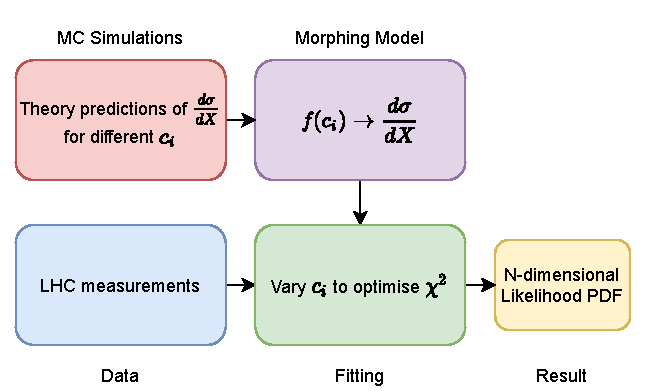
\includegraphics[width=0.75\textwidth]{images/deft-workflow.pdf}
    \caption{A diagrammatic overview of the dEFT workflow. The diagram details the steps required to obtain create a model from Monte Carlo predictions and use this model to estimate the Wilson coefficients associated with data. This process will be detailed throughout section~\ref{sec:deft}.}
\end{figure}

\subsection{Building models using linear regression}
dEFT creates predictions for the observables of interest for arbitrary values of Wilson coefficients by constructing and applying a type of model known as a linear morphing model.
A linear morphing model is a model which allows for the linear interpolation between different Monte Carlo predictions of varying parameters.
These Monte Carlo predictions are generated for different Wilson coefficient values which would be relevant for some dataset.
For dEFT's application, cross sectional SMEFT predictions are created using a simulation framework in order to create the model.
These predictions should include only relevant SMEFT operators $O_{i}$ for the observable for which the predictions are being made.
Using ($\ref{eq:smeft_cross_section}$), a linear model $\hat{\sigma}({C_i})$ is constructed using these Monte carlo prediction.
This model now allows for the prediction of some cross sectional observable for any values of Wilson coefficients pertaining to the relevant set of operators.
The morphing model could be avoided by instead using the simulation framework directly as the model but this has it's faults.
This would require a large amount of computational time to sample the model at multiple different points as cross section computations would need to be performed each time.
It also would remove the simplicity of using a single configuration file which dEFT has been built around.

The model must be validated to ensure the resulting model produces predictions which are sufficiently similar to the predictions produced by the simulation framework when considering the same coefficient values.
Additional simulated predictions are generated at coefficient values different to those used to create the model.
These differential cross section predictions are then compared to the model predictions to ensure they agree within a suitable error comparable to the statistical error on the Monte Carlo samples.
One issue with this form of validation is that any problems with the modelling of SMEFT in the simulation framework will not be seen in the validation tests.
This validation can only determine if the constructed morphing model is similar to the modelling of the simulation.

\subsection{Fitting Method}\label{sec:fitting}
Once a model has been built, estimating the Wilson coefficients of the data is possible.
Parameter estimation through fitting a model involves varying the parameters of a model and observing the response in some statistic with respect to the data.
Commonly, the parameters values which are extrema of the statistic best describe the data.
dEFT performs fitting using Monte Carlo Markov Chain (MCMC) methods which allow for estimation of a multidimensional posterior distributions of the Wilson Coefficients $P(C_{i}|y)$ using prior assumptions about their possible values.
MCMC estimates a distribution using a sampler which algorithmically sampling the distribution for varying parameters.
This sampler will form a chain of samples which when consider as a whole, will provide a discrete approximation for the posterior distribution.
MCMC methods are commonly used when sampling distributions which have a difficult analytic definition or might not even have an analytic form at all.
The posterior distribution of the Wilson coefficients is
\begin{equation}
    P(C_{i}|y) \propto Pr(C_{i}) \mathcal{L}(y|C_{i})
\end{equation}
where $Pr(C_{i})$ is the prior and $\mathcal{L}(y|C_{i})$ is a likelihood definition.
The posterior definition requires an estimation for the likelihood function $\mathcal{L}(y | C_{i})$ which is proportional the probability of obtaining some data $y$ given a set of model parameters $C_{i}$.
dEFT uses the Python package \emph{emcee}~\cite{Foreman_Mackey_2013} as its MCMC implementation.

When estimating the posterior distribution, dEFT uses the logarithm of the likelihood instead of the likelihood which has maxima for the same coefficient values.
The definition of log likelihood for binned Gaussian-distributed data with the associated model $f$ is
\begin{equation}\label{eq:likelihood}
    \ln\mathcal{L}(y | C_{i}) = -\sum\limits_{n} (y_{n} - f_{n}(C_{i})) V^{-1} (y_{n} - f_{n}(C_{i}))
\end{equation}
where $y_{n}$ is the binned cross sectional data, $V$ is the associated covariance matrix and $f_{n}(C_{i})$ is the morphing model prediction.
Note that this is the definition of the $\chi^{2}$ statistic where the covariance between bins is being considered.
There are off-diagonal elements of the covariance matrix in the these cross sectional datasets since when events are unfolded to extract the required observable, this introduces inter-correlation between the binned data.
In order for an estimation for the posterior distribution $P(C_{i} | y)$ to be made, a prior distribution $Pr(C_{i})$ is required.
This takes the form of uniform distributions defined by some minimum and maximum for each $C_{i}$ parameter.
MCMC will systematically sample throughout $C_{i}$ space building an estimation for the posterior distribution $P(C_{i}|y)$.
Properties regarding $C_{i}$ can be inferred from the resulting distributions.

An estimation for the coefficient is extracted from the approximated marginalised distribution of each operator.
These marginalised distributions are obtained by considering just a single coefficient from each of the samples.
The approximation for this single coefficient is defined by percentiles of the discrete samples.
The 50\ts{th} percentile is attributed as the value for the coefficient with the 16\ts{th} and 84\ts{th} percentile forming a 68\% credible interval about the value.
This definition allows for asymmetrical errors which can describe the measurement more faithfully than considering just the mean and variance of the samples.

Since MCMC methods are used, an approximations for the posterior distribution of $C_{i}$ is obtained rather than a single value which is common from other methods which attempt to maximise the likelihood.
It is common to find issues of reaching local maxima in these other methods which can be fairly common when using a SMEFT model due to the quadratic terms in the SMEFT cross section definition.
The use of a posterior distribution instead of a single value allows for more detailed results where the fit results can be displayed as a multidimensional histogram.

\section{Analysis}\label{sec:analysis}

This analysis examines the benefits of using 2D differential cross section measurements in a SMEFT analysis.
A 2D differential cross section refers to the cross section of a process with respect to two experimental observables.
The results are compared to outcomes when considering just a 1D differential cross section.
The main aim of a SMEFT analysis is to place constraints onto the Wilson coefficients of the SMEFT operators in order to constrain the potential occurrences of new interactions or modifications to the SM interactions.
2D differential cross sections are of interest due to the possibility of simultaneously constraining multiple operators.
A two different operator may have provide a different contribution when considering the differential cross section with respect to one observable compared to another.
This difference in responses can be used to constrain the Wilson coefficients of these operators.

The only SMEFT operators considered were $O_{tG}$ and $O_{tq}^{8}$ with corresponding Wilson coefficients $C_{tG}$ and $C_{tq}^8$.
For a more complete analysis, all relevant four fermion operators should be included but this would drastically increase the scale of computational processing and analysis.
The limited set of only two operators should still reveal the influences of changing from a single dimensional differential cross section to a multidimensional differential cross section.

This section will begin with the details of the ATLAS cross section measurements and the SMEFT cross section simulations needed to create the morphing models for determining the constraints on the Wilson coefficients.
The section will move into applying this model and obtaining estimations for the distribution of the coefficients for both the 1D observable and the two observable.

\subsection{Measurements of differential cross section of \texorpdfstring{$t\bar{t}$}{ttbar} production}
This report will use differential cross section data of top pair production from the ATLAS experiment~\cite{ATLAS:2019hxz} at the CERN Large Hadron Collider.
The data used is publicly available through HEPData~\cite{hepdata1750330}.
This data was produced from pp collisions performed at a centre-of-mass energy $\sqrt{s} = 13$TeV over the course of 2015 and 2016 with an integrated luminosity of 36.1fb$^{-1}$.
The properties of the $t\bar{t}$ system are extracted from the $\ell$+jets channel in the resolved topology where the resolved topology implies that the decay of the hadronically decaying top are well separated in angle.
This decay scheme contains a leptonically decay top with a hadronically decaying top.

The 2D differential cross section observable considered was the differential cross section as a function of the invariant mass of the $t\bar{t}$ system $m_{t\bar{t}}$ and the transverse momentum of the hadronically decaying top quark $p_{T}^{t}$.
These are the mass of the top-antitop system in its rest frame and the component of the hadronically decaying top's momentum travelling radially from the beam line in the collider.
For the comparison with a 1D observable, the differential cross section as a function of just $m_{t\bar{t}}$ was examined.
The differential cross section data for just $m_{t\bar{t}}$ may be referred to as the single or 1D obervable and the differential cross section data with respect to $m_{t\bar{t}}$ and $p_{T}^{t}$ may be referred to as the 2D observable.

The data provided contains the associated statistical and systematic uncertainties introduced during the measurements of the cross sections.
Multiple sources of systematic uncertainty are introduced in the process of measuring the $t\bar{t}$ systems.
This includes the uncertainty associated with the reconstruction of the lepton and the various jet products of the process.
There is also the uncertainty associated with the tagging of jets containing $b$-hadrons as well as accounting for possible misidentifications of jet flavour.
The uncertainty associated with the reconstruction of the missing transverse momentum $E_{T}^{\text{miss}}$ must also be accounted for.
Error in the modelling of the signal and background contributions and the Monte Carlo statistical error involved in creating these models are propagated.

Through HEPData, the covariance matrices associated with the differential cross section measurements are made available to the public.
Inter-bin correlations are introduced due to the detector effects which may cause an event to be placed in a neighbouring bin than the truth information would imply.
The analysis was initially conducted with the full covariance matrix of each data set which was implemented into the likelihood definition as seen in (\ref{eq:likelihood}).
Unfortunately, this caused the likelihood definition to produce fits which described the data very poorly compared to if only the diagonals of the matrices were considered.
For the differential cross section data with respect to $m_{t\bar{t}}$, the fit produced with the full covariance matrix had a corresponding $\chi^2$ per degree of freedom of 12.60 while this was reduced to 0.53 when only considering just the diagonal elements.
The covariance matrices provided were examined and it was found that they indicated that the bins of the histogram were very correlated for a dataset of this type.
The correlation matrix for the binned differential cross section measurement is defined as
\begin{equation}
    \textrm{corr}(\vec{x}) = \textrm{diag}(V) V \textrm{diag}(V)
\end{equation}
where $\vec{x}$ are the bins of the histogram and $V$ is the associated covariance matrix.
The correlation between bins in the 1D differential cross section histogram is shown as an example in Figure~\ref{fig:correlation}.
This shows that some bins have over 90\% correlation with other bins which are not particularly.
The magnitude of this type of correlation could not be attributed to just detector effects.
This was considered to be an error in the covariance matrix provided by HEPData and the covariance between different bins were ignored.

\begin{figure}[H]
    \centering
    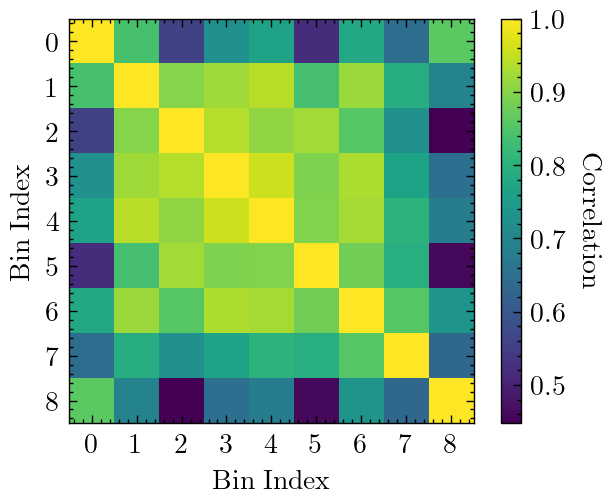
\includegraphics[width=0.5\textwidth]{plots/correlation.png}
    \caption{Correlation matrix between $m_{t\bar{t}}$ bins of histogram for the differential cross section with respect to $m_{t\bar{t}}$ dataset. All bins shows a large correlation with all other bins ranging from \textasciitilde~50\% to \textasciitilde~90\%. The diagonal elements of 1 show the correct calculation for the self correlations of bins.}
    \label{fig:correlation}
\end{figure}

\subsection{Simulation of Monte Carlo samples}
In order to build the morphing model, simulated samples were required throughout the space of Wilson coefficients for the operators of interest.
These samples were generate using the MadGraph5\textunderscore aMC@NLO~\cite{Alwall_2014} framework which allows for the simulation of processes for a user-defined Lagrangian.
The SMEFTatNLO~\cite{degrande2020automated} FEYNRULES model implements SMEFT LO and NLO processes into MadGraph5.
Though there is the capacity to perform predictions at NLO, these calculations greatly increase the processing time required to produce the Monte Carlo predictions.
This remains an area of exploration for further analysis.
The simulations were performed to fixed order which means only the desired observables of $m_{t\bar{t}}$ and ${p_{T}^{t}}$ are calculated and binned in the same binning arrangement as the ATLAS dataset of interest.

Separate sets of MC signal was required for the 1D observable and the 2D observables analyses.
Calculations were performed with 13 values of $C_{tg}$ ranging from -4 to 4 and 13 values of $C_{tq}^{8}$ from -4 to 4.
This resulted in the single operator model having 13 samples to build the model.
The two operator model using the different combination of the 13 $C_{tg}$ values and the 13 $C_{tq}^{8}$ values in order to have 169 samples.
Additional samples were also required to perform validation of the model predictions.
These samples were required to not be at the same coefficient values as the samples which were used to build the models.
The single operator model used 10 samples of varying $C_{tg}$ for validation.
The two operator model used 100 samples with varying $C_{tg}$ and $C_{tq}^{8}$.
The simulation stage imposes a great challenge when wanting to expand into using more SMEFT operators in the model.
The number of required MC samples to ensure consistent description of the parameter space increases exponentially with the number of operators.
This is a major factor in the decision to not include all top pair related 4-fermion operators in this report.
It would drastically increase the required wall time and the computational capacity.

In order for the simulated events to be comparable to the data taken from ATLAS, the uncertainty associated with the simulation must be estimated and the lowest order simulation must be scaled to be comparable to the measurements through a $k$-factor.
This process is detailed in the following subsections.

\subsubsection{Uncertainty due to simulation}\label{sec:scale_variation}

The simulation calculations conducted were required to obtain a statistical accuracy of 1\% for the prediction of the integrated cross section of top-antitop production.
This places a numerical error within the numerical integration performed when calculating the cross sections.
This is handled by an configuration parameter in the MadGraph5 event generation.
This level was considered reliable since this error was minimal in comparison to the total uncertainty of the ATLAS cross section data but still able to be computed in a reasonable time frame.
An accuracy requirement on each bin was unavailable and would have allowed for a clearer comparison to the error associated with each bin of the data.

Theoretical uncertainties on the Monte Carlo samples also needed to be accounted for.
This was done by varying the renormalisation and factorisation scales by two for the upper scale and by a half for the lower scale.
This scale variation is intended to describe contribution from higher order contributions in the theory.
The scale variation was calculated through MadGraph5 using the SMEFTatNLO model with all operators being suppress.
This provided a prediction of the scale variation effects for the Standard Model at NLO which could then be applied to SMEFT samples.
Even at NLO, these scale variation effects can influence the total cross section by between 5\% to 10\%.
This exceeds the error on the ATLAS data and the uncertainty introduced due to numerical accuracy of the simulations.

\subsubsection{Calculation of \texorpdfstring{$k$}{k}-factor}
Since the generated SMEFT predictions only included LO processes, these predictions needed to be scaled to be comparable to the necessary datasets.
It can be considered fairly accurate to compare NNLO predictions to actual cross sectional data so a method of scaling the current predictions to this level is required.
NNLO is considered to be a sufficient order since performing the theoretical calculation beyond this becomes very difficult.
Due to the difficulty in calculating the $k$-factor for different combinations of Wilson coefficients values, the $k$-factor for the Standard Model prediction was used across the various SMEFT predictions.

A flat $k$-factor across the differential cross sections was attempted to bring the LO predictions to the scale of NNLO predictions using the proportions between LO calculations of total cross section from MadGraph5 and the predicted total cross section up to NNLO which was calculated using the Top++2.0 program~\cite{Czakon:2011xx}.
This method failed due to some regions of the differential cross sections being poorly described at LO which caused a flat scaling to incorrectly describe the shape of the distributions at NNLO.
This is exemplified by the low $m_{t\bar{t}}$ and high $p_{T}^{t}$ region in the two observable data set, as seen in Figure~\ref{fig:kfactor}.
This is remedied by requiring a per-bin $k$-factor when scaling from LO to NLO but still using the flat factor to build up to NNLO.
The per-bin $k$-factor was found by comparing the Standard Model predictions of MadGraph5 at LO and NLO and applying this ratio to the Monte Carlo signal.

\begin{figure}[H]
    \centering
    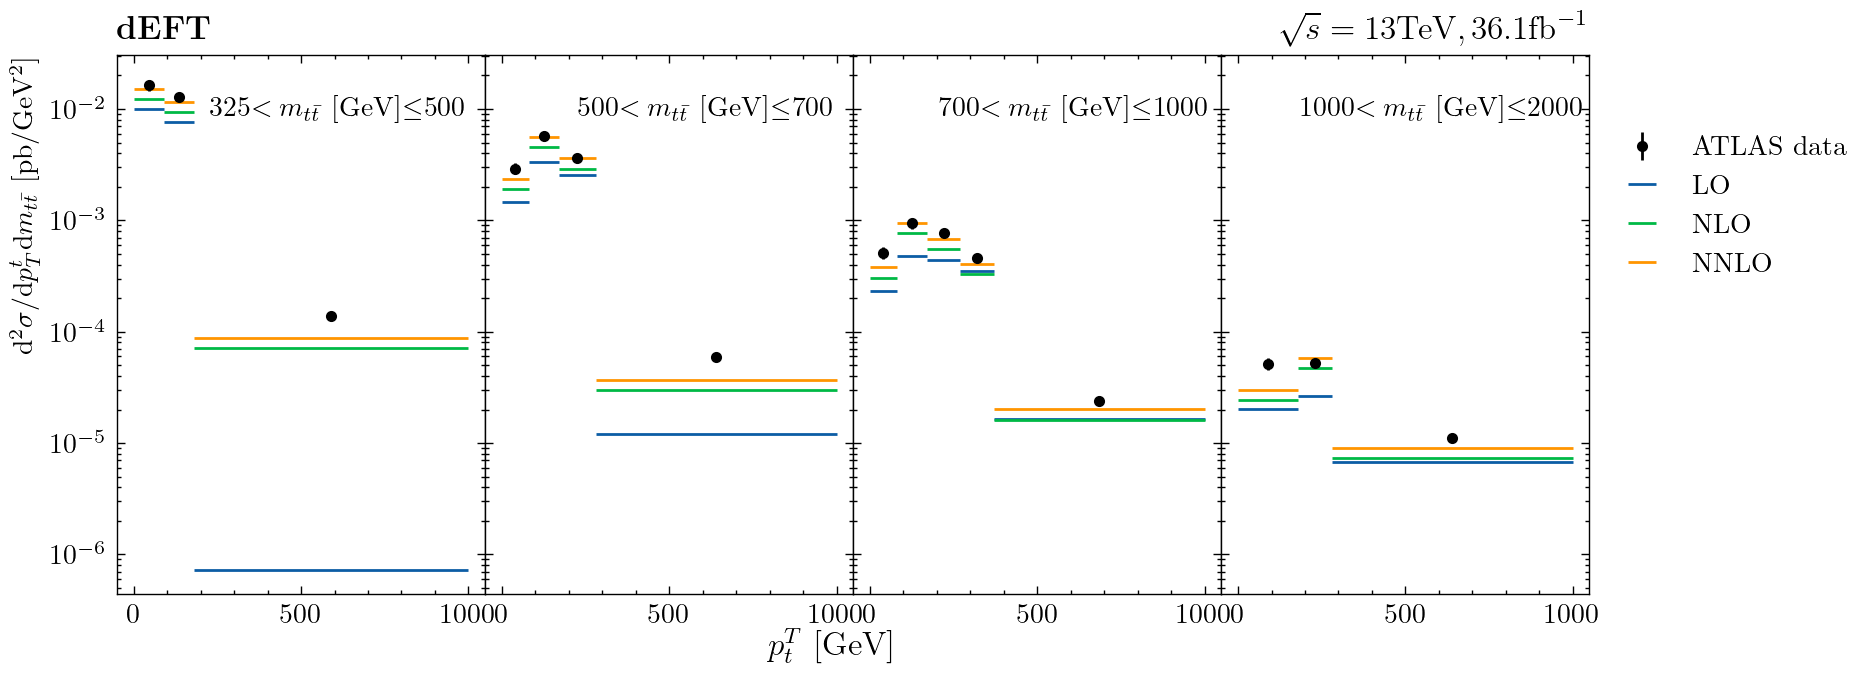
\includegraphics[width=\textwidth]{plots/k_factor.png}
    \caption{Comparison of estimations of absolute 2D differential $t\bar{t}$ cross section with respect to $m_{t\bar{t}}$ and $p_{T}^{t}$ to varying orders. The 2D bins are shown with each panel describing a different $m_{ttbar}$ bin in which the $p_{t}^{T}$ bins are shown. The scaling from an LO approximation (blue) to an NLO approximation (green) was determined using a per-bin method and the NNLO prediction (orange) was determined using a flat factor. The associated ATLAS data is also included for comparison.}
    \label{fig:kfactor}
\end{figure}

The theoretical error associated with the calculated $k$-factor is fairly difficult to propagate through the model construction and should be dominated by the error associated with the data.
This may have consequences on bins which are not well described at LO though the scale variances should dominate the uncertainties introduced by the $k$-factor.

\subsubsection{Response to operators}\label{sec:response}

With a set of observables declared, simulated samples were used to examine the response of $t\bar{t}$ differential cross sections when the associated Wilson coefficients were varied in the theory.
Various theoretical predictions for cross section are shown in Figure~\ref{fig:comparison}.
Focussing on the response with respect to $C_{tG}$, there appears be a general normalisation effect on the majority of bins of the distribution.
This provides a clear interpretation of the operator but exposes some issues in estimating $C_{tG}$.
If $O_{tG}$ is related to a scaling of the distribution, any other contribution which scales the theoretical predictions may impact the estimation of $C_{tG}$.
This would include the $k$-factor used to ensure the leading order MC predictions are comparable to the data.

The operator $C_{tq}^{8}$ has a more varied response across the distribution.
It appears that the effects of $O_{tq}^{8}$ are more prominent at the higher regions of transverse momentum of the hadronically decaying top $p_{T}^{t}$.
A major difference between the response in $C_{tq}^{8}$ and $C_{tG}$ is that an increasing $C_{tq}^{8}$ does not uniformally increase of cross section.
This non-uniformity in how the bins transform could lead to posterior distributions for the Wilson coefficients which aren't necessarily Gaussian.
If these effects are considered when modelling, it is expected that $C_{tq}^{8}$ may experience multiple optimised values which will be seen as a distribution with multiple peaks.

\begin{figure}[H]
    \centering
    \begin{subfigure}[b]{\textwidth}
        \centering
        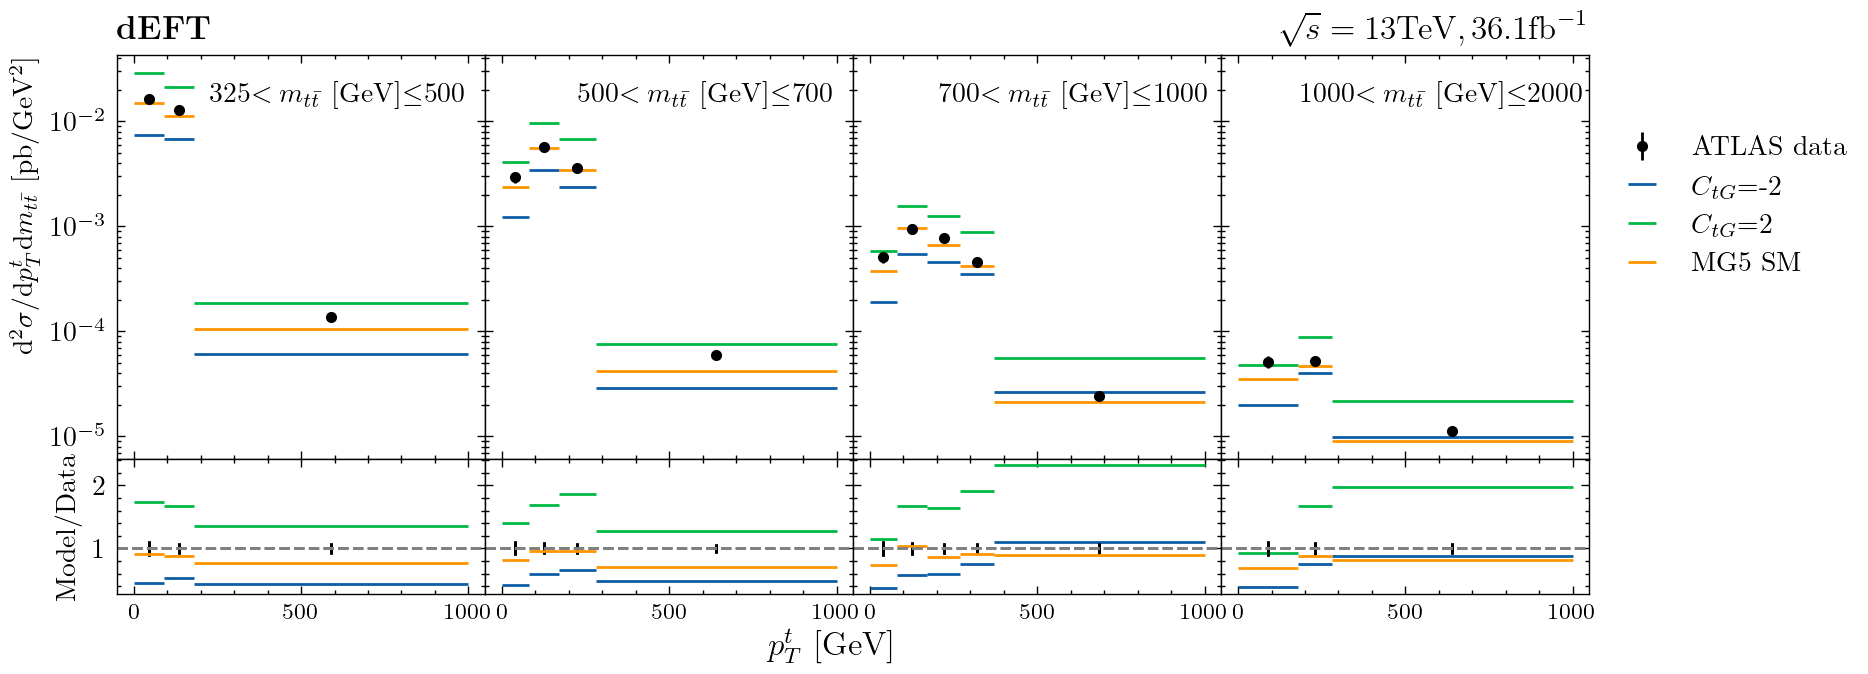
\includegraphics[width=\textwidth]{plots/data_plot_ctg.png}
        \caption{Response to $C_{tG}$}
    \end{subfigure}

    \begin{subfigure}[b]{\textwidth}
        \centering
        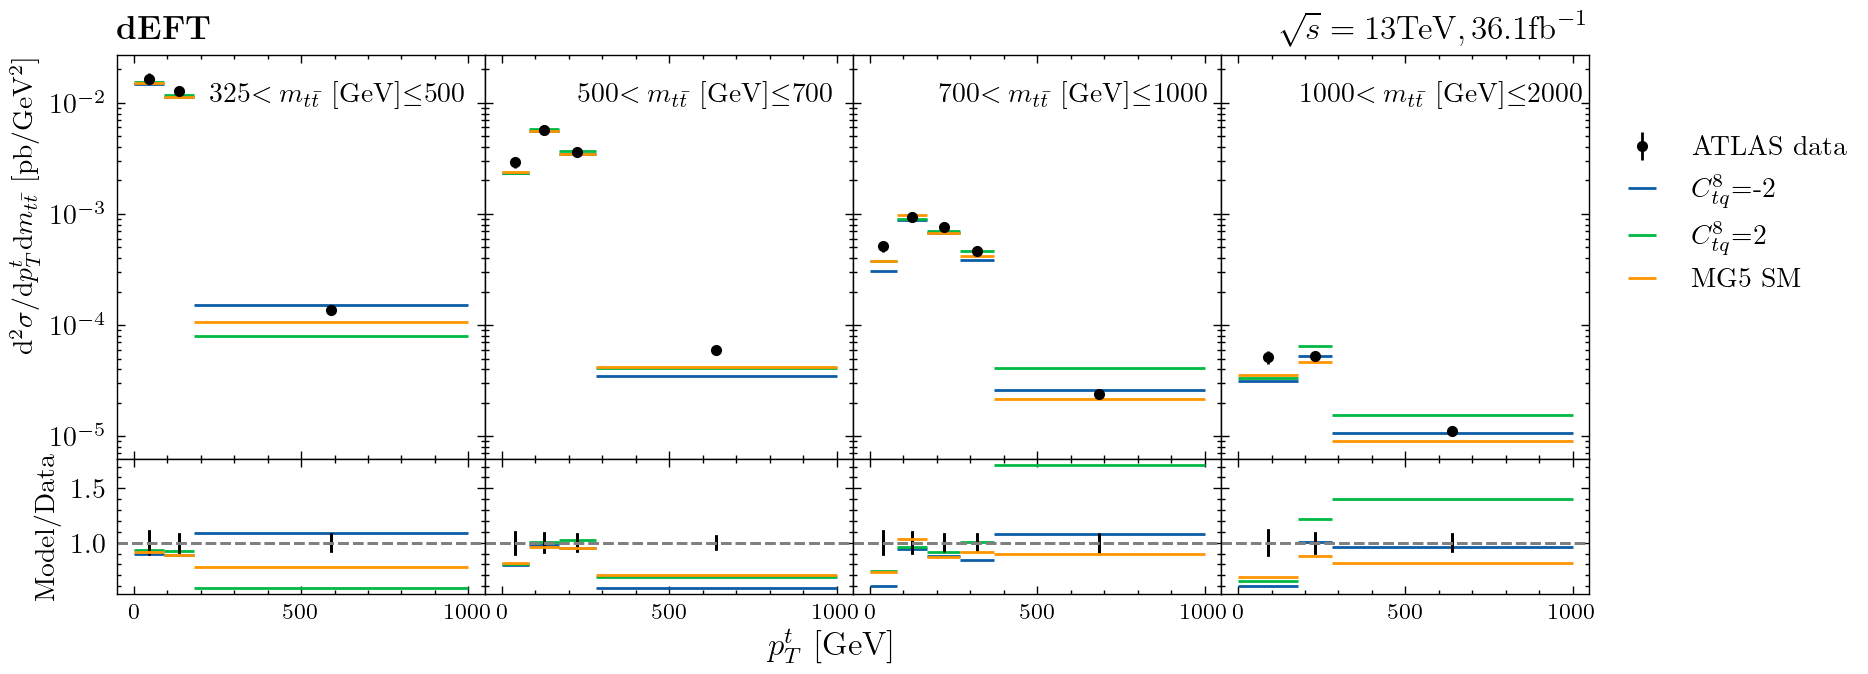
\includegraphics[width=\textwidth]{plots/data_plot_ctq.png}
        \caption{Response to $C_{tq}^{8}$}
    \end{subfigure}
    \caption{Comparison of simulated theoretical predictions of 2D differential cross section of $t\bar{t}$ production as a function of $m_{t\bar{t}}$ and $p_{t}^{T}$ for varying values of $C_{tG}$ and $C_{tq}^{8}$. The ATLAS measurements are also shown.}
    \label{fig:comparison}
\end{figure}
\todo{extend caption}

\subsection{Single operator model}\label{sec:analysis_one_op}

As a test of method, two model were constructed considering only the $O_{tG}$ operator and applied to the 1-dimensional and 2-dimensional differential cross section measurements.
Results for this analysis will show the ability for dEFT to generate a successful model using the Monte Carlo samples.
Since both the 1D and 2D differential cross section are influenced by the distribution of mass of $t\bar{t}$ system, both datasets contribute the same information to the fitting procedure.
The 2D cross section will provide more information regarding the distribution of $p_{T}^{t}$.
A separate model was created for the 1D and the 2D datasets which then required separate sets of Monte Carlo samples.
When these samples were generated, the value of the coefficient $C_{tG}$ were varied and the value of coefficient $C_{tq}^{8}$ was set to 0.

\subsubsection{Model Validation}

The models used were created using Monte Carlo samples which subject to statistical uncertainty in the simulation process.
For the model to be considered, the model should provide predictions of other statistically independent samples with a similar degree of certainty.
This deviation is expected to be comparable to the 1\% required accuracy for integrated cross section imposed MadGraph5.
Note that this is accuracy is applied on each bin of the cross sections but across the entire distribution.

The validation of the models each required 10 validation MC statistically independent samples of varying $C_{tG}$ for the 1-dimensional and the 2-dimensional cross section models.
In order to compare the validation tests to the statistical simulation accuracy, the average relative residuals between the validation samples and the models' prediction for the associated coefficient values were considered.
The average relative residuals is the summation of the relative difference of each bin between the model and the sample in each test divided by the total number of bins across all tests.
The standard deviation of this value should be the required accuracy of the simulation.

An example of a validation test where $C_{tg}=-2.0$ can be seen in Figure~\ref{fig:test_example}.
All model predictions across the bins in the tests deviate no more than 5\% from the MC sample provided by MadGraph5.
For most of the tests, the deviations per bin do exceed the 1\% accuracy required for the simulation for some bins.
The average relative residuals allows for a more general estimation of the performance of the models predictive capacity where per-bin deviation are ignored to see overall deviation from simulation.

\begin{figure}[htb]
    \centering
    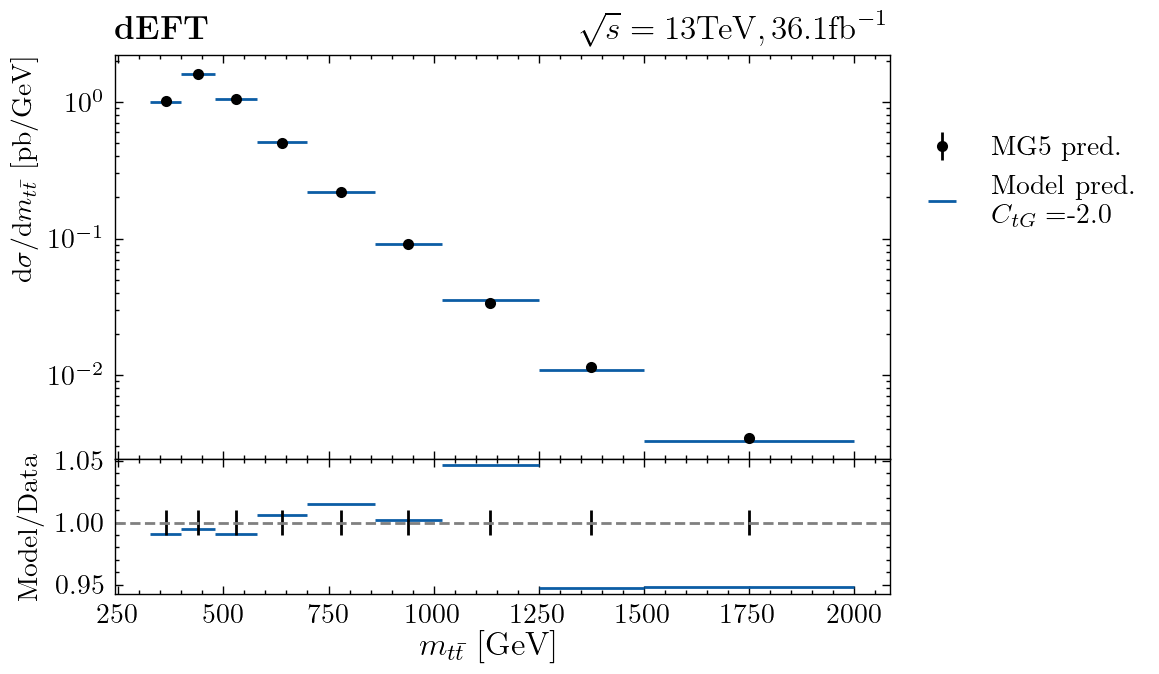
\includegraphics[width=0.9\textwidth]{plots/validation_ATLAS-ctg_2_1D_1OP.png}
    \caption{Example of validation test for the one observable model for the 1D differential cross section with for $C_{tG}=-2$. The model prediction for $C_{tG}=-2$ is compared to the simulated prediction created by Madgraph5 with $C_{tG}=-2$. The error bars shown represent a 1\% deviation on the MadGraph5 prediction. The ratio between the bins of the model and the simulation prediction is shown below.}
    \label{fig:test_example}
\end{figure}

The average relative residuals with the associated standard deviation is $0.10\pm1.21\%$ for the 1D observable model and $0.35\pm1.30\%$ for the 2D observable model.
The results of the validation tests show that both models provide very small deviation compared to the Monte Carlo sample and is comparable to the uncertainty introduced by the statistical error associated with the Monte Carlo samples.

\subsubsection{Uncertainty due to scale variation}
The theoretical uncertainty related to the Monte Carlo samples are encapsulated by the upper and lower bound of the scale variation as mentioned in Section~\ref{sec:scale_variation}.
This uncertainty is estimated through the building the model using simulation samples with adjusted scale variation.
These new models will then be fitted to the ATLAS data.
The Monte Carlo samples are adjusted to the upper and lower scale which will provide two sets of results for the posterior distributions for the Wilson coefficients.
These results can be used as bounds to estimate the systematic uncertainty of the Wilson coefficients introduced by the theoretical variation in the simulated samples.
The uncertainty of $C_{tG}$ associated with the scale variation of the Monte Carlo samples for the 1-dimensional model is $^{+0.07}_{-0.06}$ and for the 2-dimensional model is $^{+0.16}_{-0.16}$.

\subsubsection{Results}
The estimated posterior distributions created during the fitting procedure for the 1-dimensional observable and the 2-dimensional observable are shown in Figure~\ref{fig:corner_1OP}.
The results for the fits of both observable types produced posterior distributions with a similar Gaussian shape.
The estimation for the Wilson coefficients using the 1D differential cross section was $C_{tG}=0.46^{+0.08}_{-0.09}(data.)^{+0.07}_{-0.06}(pred sys.)$ and using the 2D differential cross section, the obtained estimate was $C_{tG}=0.47^{+0.05}_{-0.05}(data.)^{+0.16}_{-0.16}(pred sys.)$.
The resulting prediction for the 1D and 2D differential cross section models is shown in Figure~\ref{fig:model_result_1OP}.
These predictions show that the optimised estimate for $C_{tG}$ provides better prediction of the data for both models then the SM prediction of the models.
The $\chi^{2}$ per degree of freedom statistic for these predictions with respect to their data quantify the goodness of fit.
The 1D observable model predictions has an associated $\chi^{2}$ per degree of freedom of 1.2 for the SMEFT prediction corresponding to $C_{tG}=0.46$ and 3.16 for the SM prediction.
For the 2D observable model, the $\chi^{2}$ per degree of freedom was 2.53 for the SMEFT prediction corresponding to $C_{tG}=0.46$ and 5.60 for the SM prediction.

\begin{figure}[htb]
    \centering
    \begin{subfigure}[b]{0.3\textwidth}
        \centering
        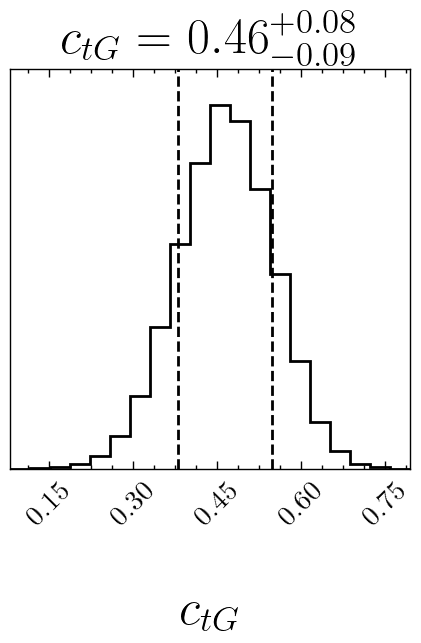
\includegraphics[width=\textwidth]{plots/ATLAS-ctg_1D_1OP.png}
        \caption{1-Dimensional Observable}
    \end{subfigure}
    ~
    \begin{subfigure}[b]{0.3\textwidth}
        \centering
        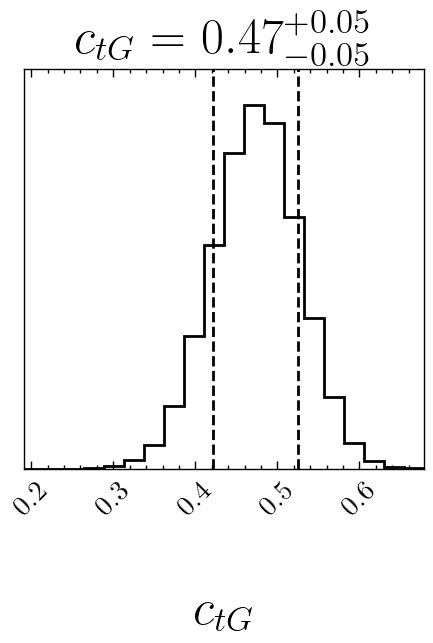
\includegraphics[width=\textwidth]{plots/ATLAS-ctg_2D_1OP.png}
        \caption{2-Dimensional Observable}
    \end{subfigure}
    \caption{Estimation for the posterior distribution for the Wilson coefficient $C_{tG}$. The dotted lines on distributions represent a 68\% credible interval. Uncertainty estimates for the Wilson coefficients are discussed in Section \ref{sec:fitting} and the errors shown on the plot only represent the statistical error due to the fit.}
    \label{fig:corner_1OP}
\end{figure}

\begin{figure}[htb]
    \centering
    \begin{subfigure}[b]{0.8\textwidth}
        \centering
        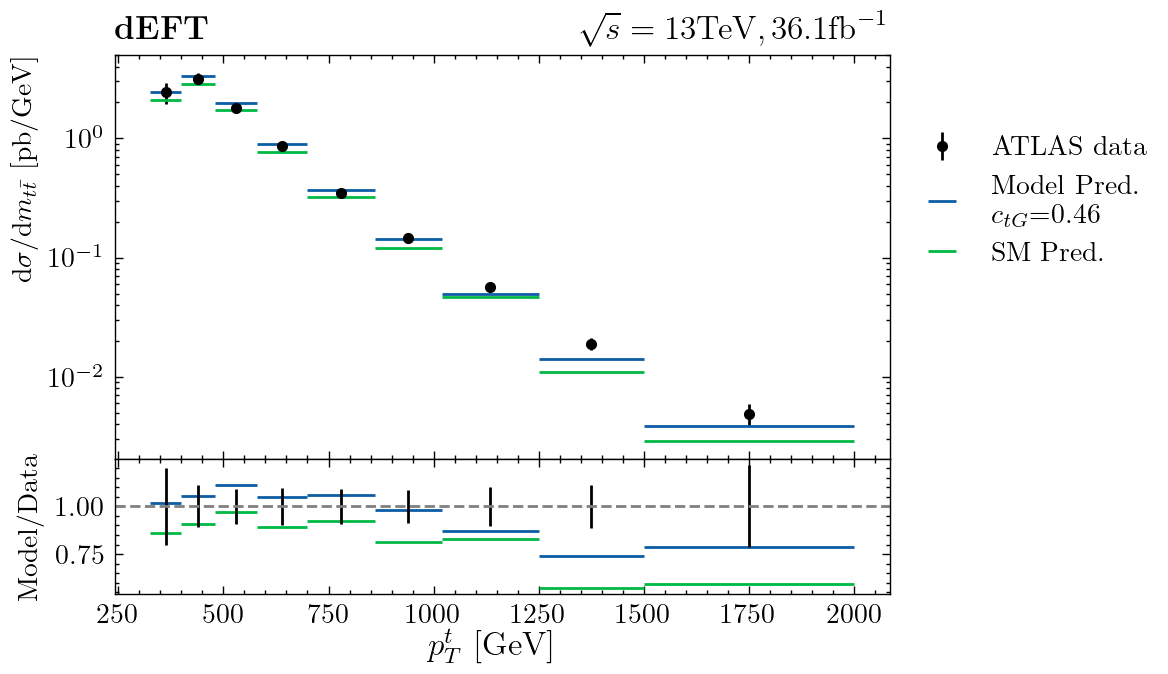
\includegraphics[width=\textwidth]{plots/ATLAS_model_result_1D_1OP.png}
        \caption{1-Dimensional observable model}
    \end{subfigure}
    \par\bigskip
    \begin{subfigure}[b]{\textwidth}
        \centering
        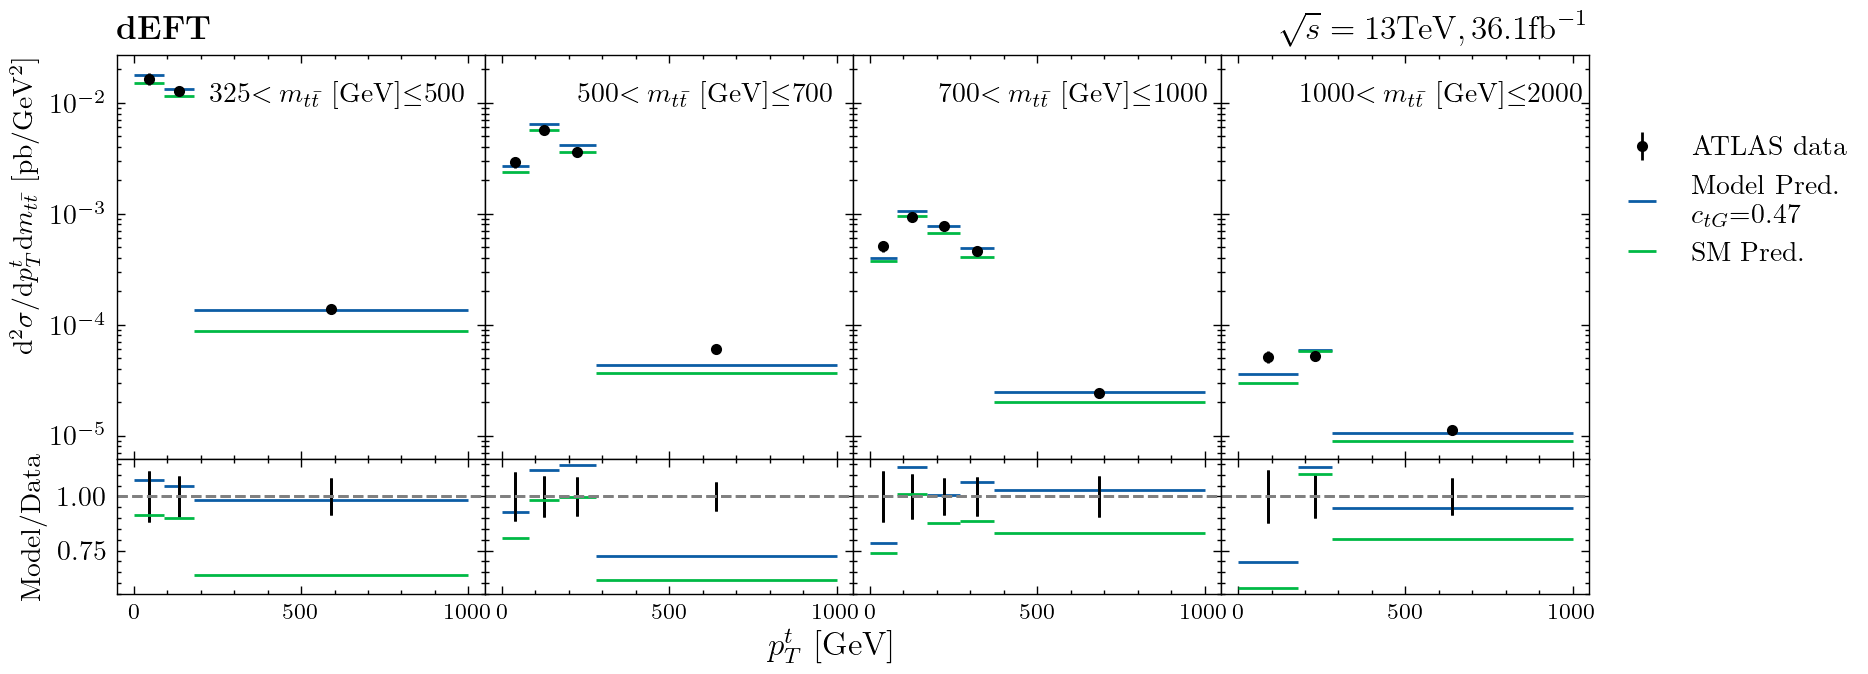
\includegraphics[width=\textwidth]{plots/ATLAS_model_result_2D_1OP.png}
        \caption{2-Dimensional observable model}
    \end{subfigure}
    \caption{Predictions of $m_{t\bar{t}}$ differential cross section measurements using two models at the optimised value of the model parameter with respect to the respective ATLAS datasets. The data used to perform the fit and the models' predictions for the SM are also shown.}
    \label{fig:model_result_1OP}
\end{figure}

The estimations for the optimised value of $C_{tG}$ for the models agree within a 68\% confidence interval and provides some interesting points of comparison.
The statistical uncertainty associated with the measurement is lower for the 2D differential cross section model.
This means that even though there are increased relative errors on the bins for 2D differential cross sections measurements than for 1D differential cross sections, the 2D observable model provides tighter constraints on $C_{tG}$ than the 1D observable model.
This may indicate that using this 2D observable would allow for better constraints on Wilson coefficients in SMEFT analyses.
A caveat arises when the systematic uncertainty is considered.
The systematic uncertainty is larger when using the 2D observable which may indicate that the bins which are allowing for the greater constraint of the coefficient may be more affected by the scale variation.
This indicates that this increase in the ability to constrain the coefficient may expose regions which are not well modelled by the theoretical predictions.

\subsection{Two operator model}\label{sec:analysis_two_op}

The software and techniques for the single operator analysis could then be used to introduce another operator $O_{tq}^{8}$ as well as $O_{tG}$.
This additional operator increases the scope of the analysis since more Monte Carlo samples are required to sufficiently describe this now 2-dimensional parameter space of the models.
The estimation of posterior distributions of the coefficients produced by the MCMC methods are now 2-dimensional and expose any correlations between the fitted parameters.

\subsubsection{Model Validation}

The results of the validation testing for both models can be seen in Figure~\ref{fig:residuals_hist} where deviations between the model predictions and the validation samples are shown by the average relative residuals.
The tests for the 1D observable model appear to follow an accuracy of 1.09\% which is in-line with the expectation from the event generation.
The average relative residuals for the 2D observable model appear to be distributed by a normal distribution as well but with a deviation of 1.68\%.
This result is larger than the validation deviation of the single obervable but is still comparable to the statistical accuracy of the MC samples.
When considering the results across all validation tests, both models appeared to provide sufficient agreement with the MadGraph5 samples and were used for estimating the distributions of the Wilson coefficients.

\begin{figure}[H]
    \centering
    \begin{subfigure}[b]{0.4\textwidth}
        \centering
        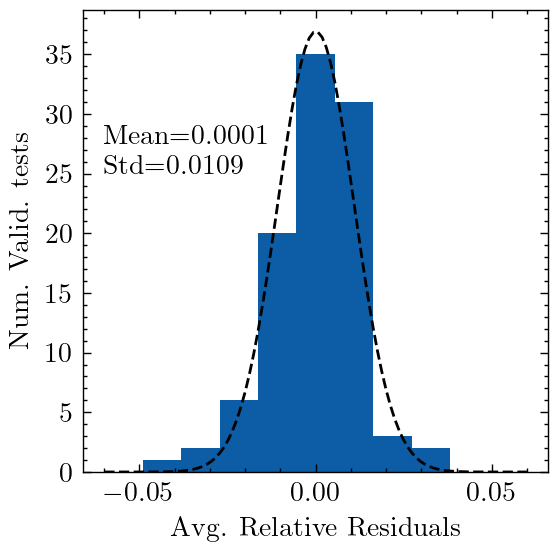
\includegraphics[width=\textwidth]{./plots/residuals_hist_1D.png}
        \caption{1-Dimensional Observable}
    \end{subfigure}
    ~
    \begin{subfigure}[b]{0.4\textwidth}
        \centering
        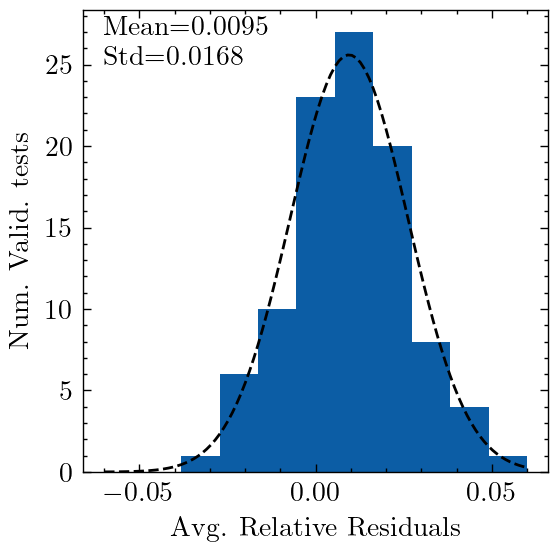
\includegraphics[width=\textwidth]{./plots/residuals_hist_2D.png}
        \caption{2-Dimensional Observable}
    \end{subfigure}
    \caption{Distribution of average relative residuals between model predictions at some set of coefficient values and the corresponding MC validation sample for each model. Each entry of the histogram is the average relative residuals for a single validation test. This includes the validation tests over 100 different validation points. The dotted line represents a Gaussian fit to the histogram through $\chi^2$ minimisation with the results of the fit shown.}
    \label{fig:residuals_hist}
\end{figure}

\todo{maybe include example validation plots}
\subsubsection{Results}

The estimations for the 2D likelihood distributions for the Wilson coefficients generated by each model are shown in Figure~\ref{fig:corner_2OP}.
It should be noted that the expansion of the parameter space to 2 operators has allowed for the description of the distribution in the form of a 2D likelihood distribution as well as a marginal distribution for each coefficient.
First, the results of the 1D observable analysis using two operators will be detailed.

\paragraph{1D observable model}

The posterior distribution created through fitting the 1D observable model to data provided estimates of $C_{tG}=0.24^{+0.11}_{-0.11}$ and $C_{tq}^{8}=1.56^{+0.25}_{-0.31}$ where these estimates are only considering statistical uncertainty of the distribution due to the fitting procedure.
A notable features of the marginal $C_{tq}^{8}$ distribution is a large peak at $C_{tq}^{8}\approx-2.5$ second less prominent peak located at $C_{tq}^{8}\approx-2.5$.
This is a product of the quadratic nature of the SMEFT model and is a behaviour which is expected when considering the response of the differential cross section with respect to $m_{t\bar{t}}$ as discussed in section~\ref{sec:response}.
The major peak in the distribution appears to show a negative correlation between $C_{tg}$ and $C_{tq}^8$.
This could be a result of the overall scaling introduced by $O_{tg}$ correlating with the scaling on some bins caused $O_{tq}^{8}$.

The model created using the upper bound of the scale variation of the MC signal produced an estimation of $C_{tG}=0.21$ and $C_{tq}=1.33$.
The lower bound of the scale variation of the MC signal produced an estimation of $C_{tG}=0.27$ and $C_{tq}=1.78$.
\todo{should I consider uncertainty on these values?}
This implies a resulting systematic uncertainties introduced due to the scale variation of the simulated data of $\pm 0.03$ for $C_{tG}$ and $^{+0.22}_{-0.23}$ for $C_{tq}^{8}$.

The 1D observable analysis obtained an estimate for the Wilson coefficients of $C_{tg} = 0.24 \pm 0.11 (data) \pm 0.03 (pred sys.)$ and $C_{tq}^{8}=1.56^{+0.25}_{-0.31} (data) ^{+0.22}_{-0.23} (pred sys.)$.
The model prediction for this estimation can be seen in Figure~\ref{fig:model_result_1D_2OP}.
The predictions from the model at the optimised coefficients appears to better describe the data compared to using the SM prediction from the model.
The optimised prediction corresponded to a $\chi^{2}$ per degree of freedom of 0.54 with respect to the data while the all zero prediction corresponded to a $\chi^{2}$ per degree of freedom of 3.16 indicating that the optimised prediction better describes the data.

When these coefficient estimations are compared with those obtained when using the single operator model, there is an agreement with the value of $C_{tG}$ when considering both the statistical uncertainty of the fits and systematic uncertainty introduced by the scale variation.
However, the estimation of $C_{tq}^{8}$ in the fit using the two operator model deviates greatly from the assumed value of $C_{tq}^{8}=0$ for the single operator models and for SM predictions.

This does provide some interest in possibly applying constraints beyond the Standard Model but there are some faults with this consideration.
The systematic uncertainty associated with the model creation and prediction was not accounted for in the uncertainty estimation.
Since these influences will equally be present when considering the 2D differential cross section data, this discussion will be deferred to later sections and these results will be used as a point of comparison between single and two observables analyses.

\begin{figure}[htb]
    \centering
    \begin{subfigure}[b]{0.45\textwidth}
        \centering
        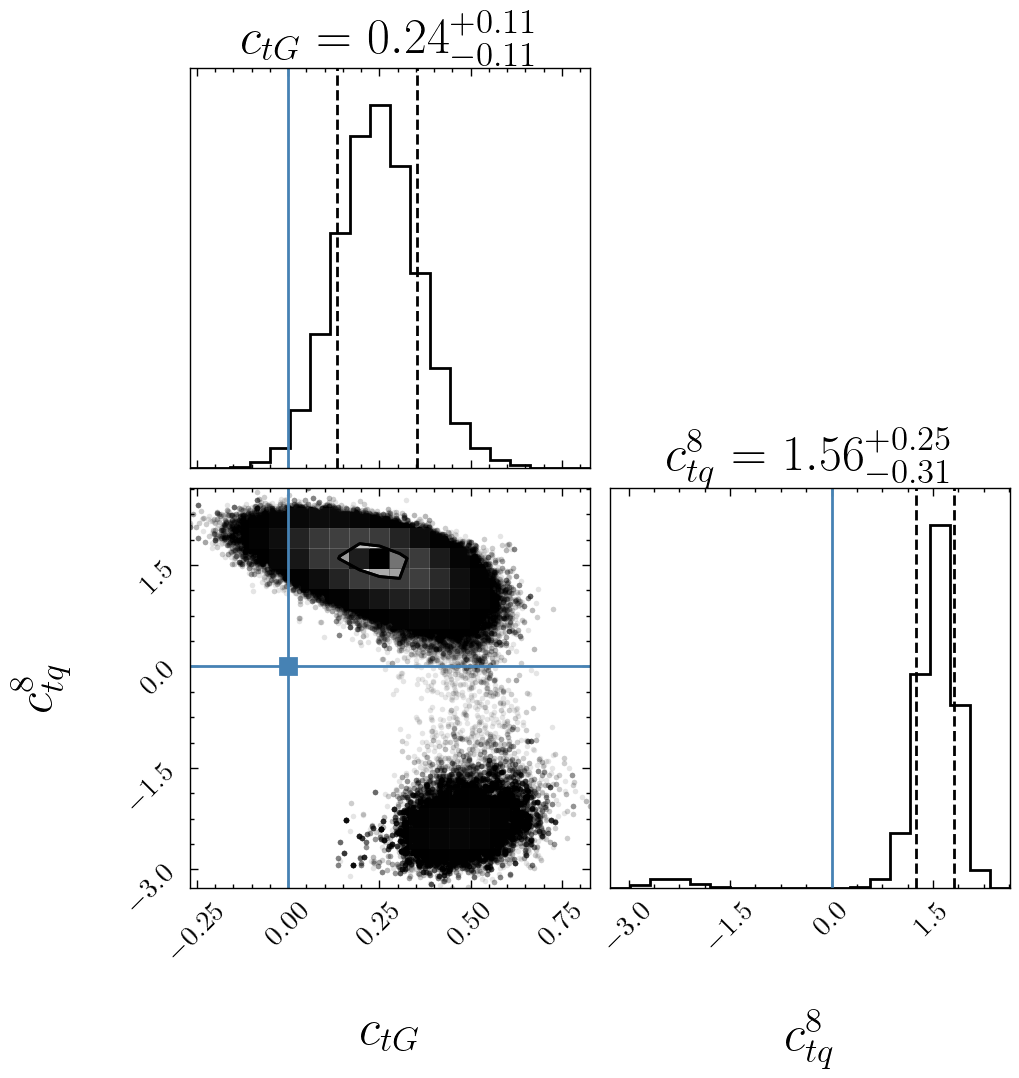
\includegraphics[width=\textwidth]{plots/ATLAS-ctg-ctq8_1D_2OP.png}
        \caption{1-Dimensional Observable}
        \label{fig:corner_1D_2OP}
    \end{subfigure}
    ~
    \begin{subfigure}[b]{0.45\textwidth}
        \centering
        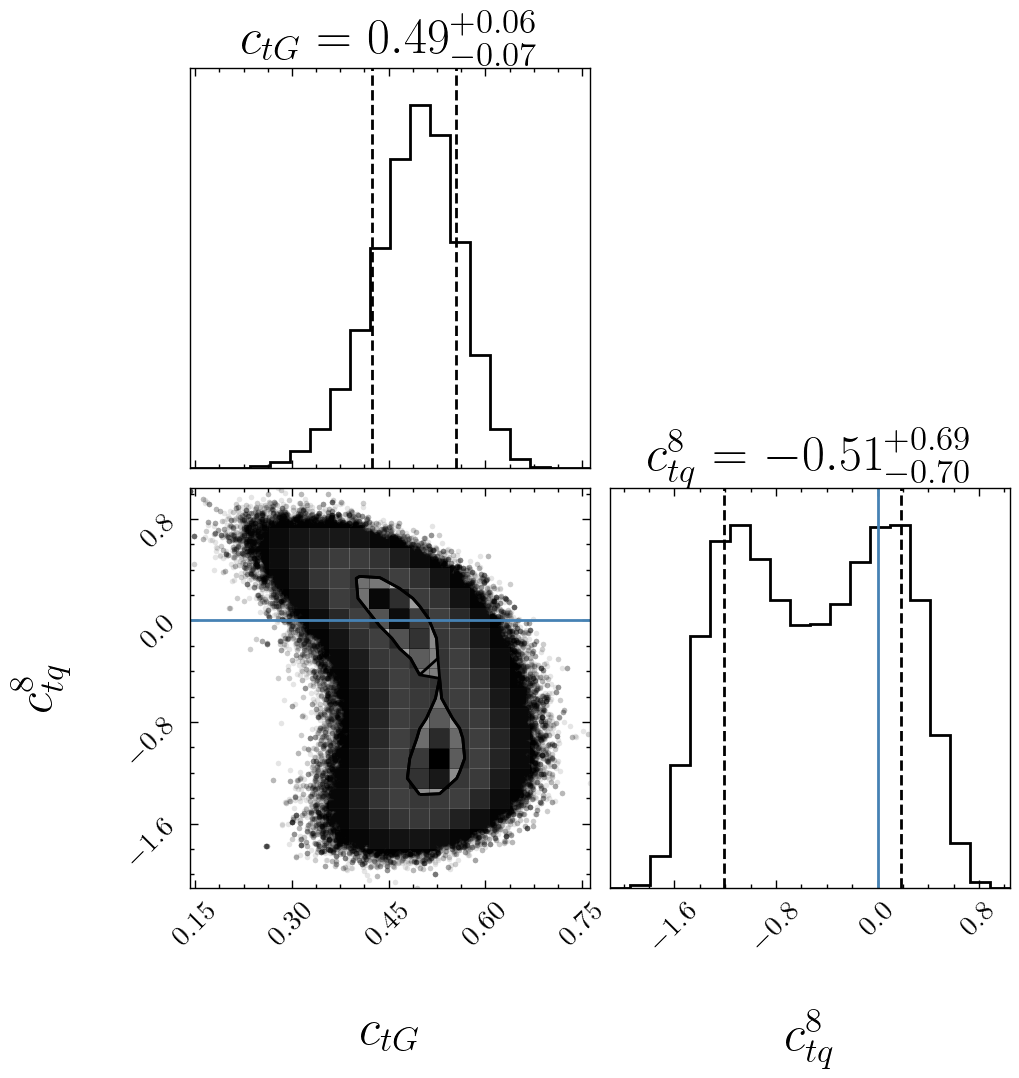
\includegraphics[width=\textwidth]{plots/ATLAS-ctg-ctq8_2D_2OP.png}
        \caption{2-Dimensional Observable}
        \label{fig:corner_2D_2OP}
    \end{subfigure}
    \centering
    \caption{Estimation for the 2D posterior distribution and 1D marginal distributions for the Wilson coefficient $C_{tG}$ and $C_{tq}^{8}$ obtained by fitting each model onto the respective ATLAS differential cross section measuremnts. The blue lines represent SM predictions. The dotted lines on the marginal distributions represent a 68\% confidence interval. Uncertainty estimates for the Wilson coefficients are discussed in Section \ref{sec:fitting} and the uncertainty on the plot show only the statistical uncertainty introduced by the fit.}
    \label{fig:corner_2OP}
\end{figure}

\paragraph{2D observable model}

The 2D observable analysis when considering the two operators provided results which fall more in line with the results found for the single operator case.
The distributions produced through the MCMC method have estimates of the Wilson coefficient values of $C_{tG}=0.49_{-0.07}^{+0.06}$ and $C_{tq}^{8}=-0.51_{-0.70}^{+0.69}$.
It can be seen that the 2D observable model applies better constraints of statistical uncertainty on $O_{tG}$ similar to what occurred for the 1D observable model.
The shape of the distribution shows a more prominent double peak structure compared to what was seen in the 1D observable analysis for two observables.
This makes interpreting the value of the coefficients fairly difficult. \todo{more detail}

These two peaks provide two optimised values which would maximise the likelihood which isn't fully compatible with the percentile definitions of the best fit value and uncertainty which has been used for evaluating the optimised coefficient values for the other models.
In order to extract the estimations provided by each of these peaks, a more traditional likelihood maximisation algorithm through the L-BFGS algorithm provided through SciPy~\cite{2020SciPy-NMeth} was used.
The two maximums were determined by providing different initial conditions for each peak.
The uncertainty on these estimates were obtained by using the inverse Hessian matrix provided by the algorithm implementation.
The estimation for the points of maximum likelihood are $C_{tq}^{8\,(1)}=-1.14\pm0.39$ and $C_{tq}^{8\,(2)}=0.10\pm0.37$.
This provides a solution $C_{tq}^{8\,(2)}$ which agrees with zero and therefore is consistent with the SM prediction and the single operator model result for the 2D observable.
Since the SMEFT does allow these multiple peaks, the entire distribution should be considered and the estimation found using percentiles will be considered further.
If more operators were included in some analysis, another coefficient could suppress one of these peaks and provide a clear measurement of $C_{tq}^{8}$.

The estimated systematic uncertainty associated with the scale variation of the simulated samples is $^{+0.11}_{-0.13}$ for $C_{tG}$ and $^{+0.21}_{-0.87}$ for $C_{tq}^{8}$. \todo{maybe change to table}
The final estimation for the Wilson coefficients using the percentile definition for the $t\bar{t}$ differential cross section with respect to $m_{t\bar{t}}$ and $p_{T}^{t}$ are $C_{tG} = 0.49_{-0.07}^{+0.06}(stat) ^{+0.11}_{-0.13} (sys.)$ and $C_{tq}^{8}=-0.51_{-0.70}^{+0.69} (stat.) ^{+0.21}_{-0.87} (sys.)$.
The model prediction for this estimation can be seen in Figure~\ref{fig:model_result_2D_2OP}.
The fitted parameters provide a better goodness of fit with respect to the data compared to SM predictions of the model with the fitted values corresponding to a $\chi^{2}$ per degree of freedom of 2.76 while the SM predictions resulted in a $\chi^{2}$ per degree of freedom of 5.60.

Both of the peak solutions do not agree with the optimal parameter found for the single operator model within statistical uncertainty.
This suggests that that the result for the 1D observable is describing some qualities of the cross sectional distribution which is not present when the 2D observable is considered.
This is extremely interesting since it indicates that the method for model creation used can generate models which produce estimations for the coefficients which are not consistent between the 1D differential cross section and the 2D differential cross section.
A possible reason for this discrepancy may be due to the modelling of $C_{tq}^{8}$ and the ability for the morphing model creation to describe the operator's relationship to $\frac{\partial \sigma}{\partial m_{t\bar{t}}}$.
The use of a 2D differential cross section may expose more information needed for the model creation which is integrated out when looking at the single differential.


\begin{figure}[H]
    \centering
    \begin{subfigure}[b]{0.8\textwidth}
        \centering
        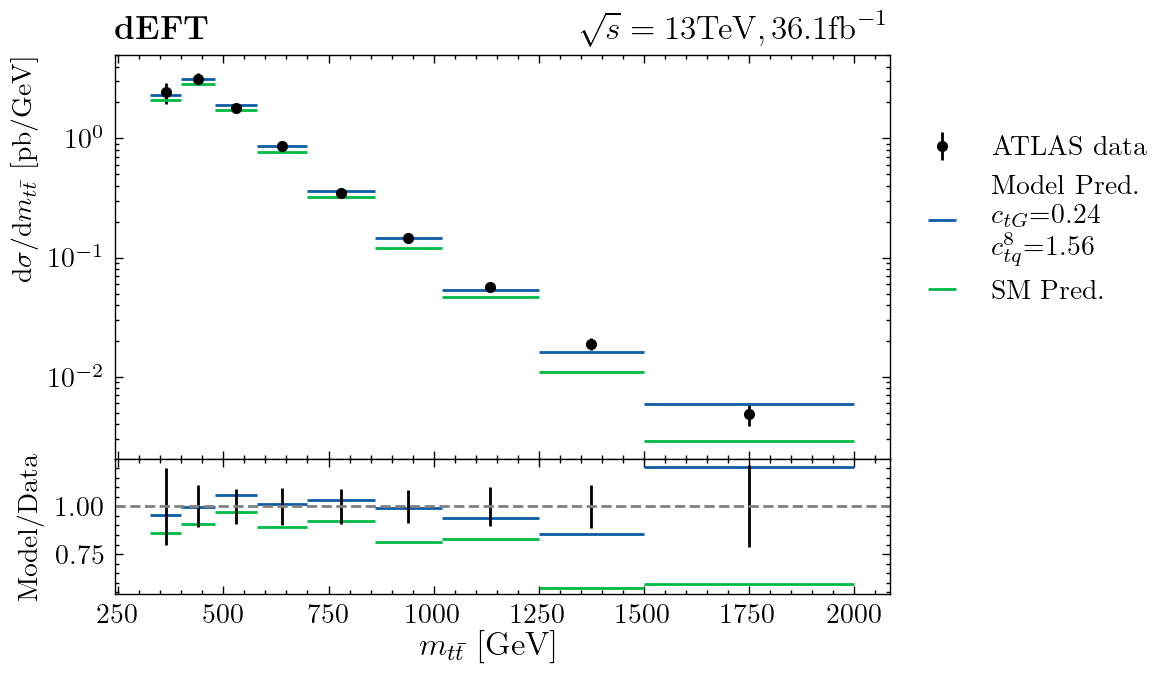
\includegraphics[width=\textwidth]{plots/ATLAS_model_result_1D_2OP.png}
        \caption{1-Dimensional Observable}
        \label{fig:model_result_1D_2OP}
    \end{subfigure}
    ~
    \begin{subfigure}[b]{\textwidth}
        \centering
        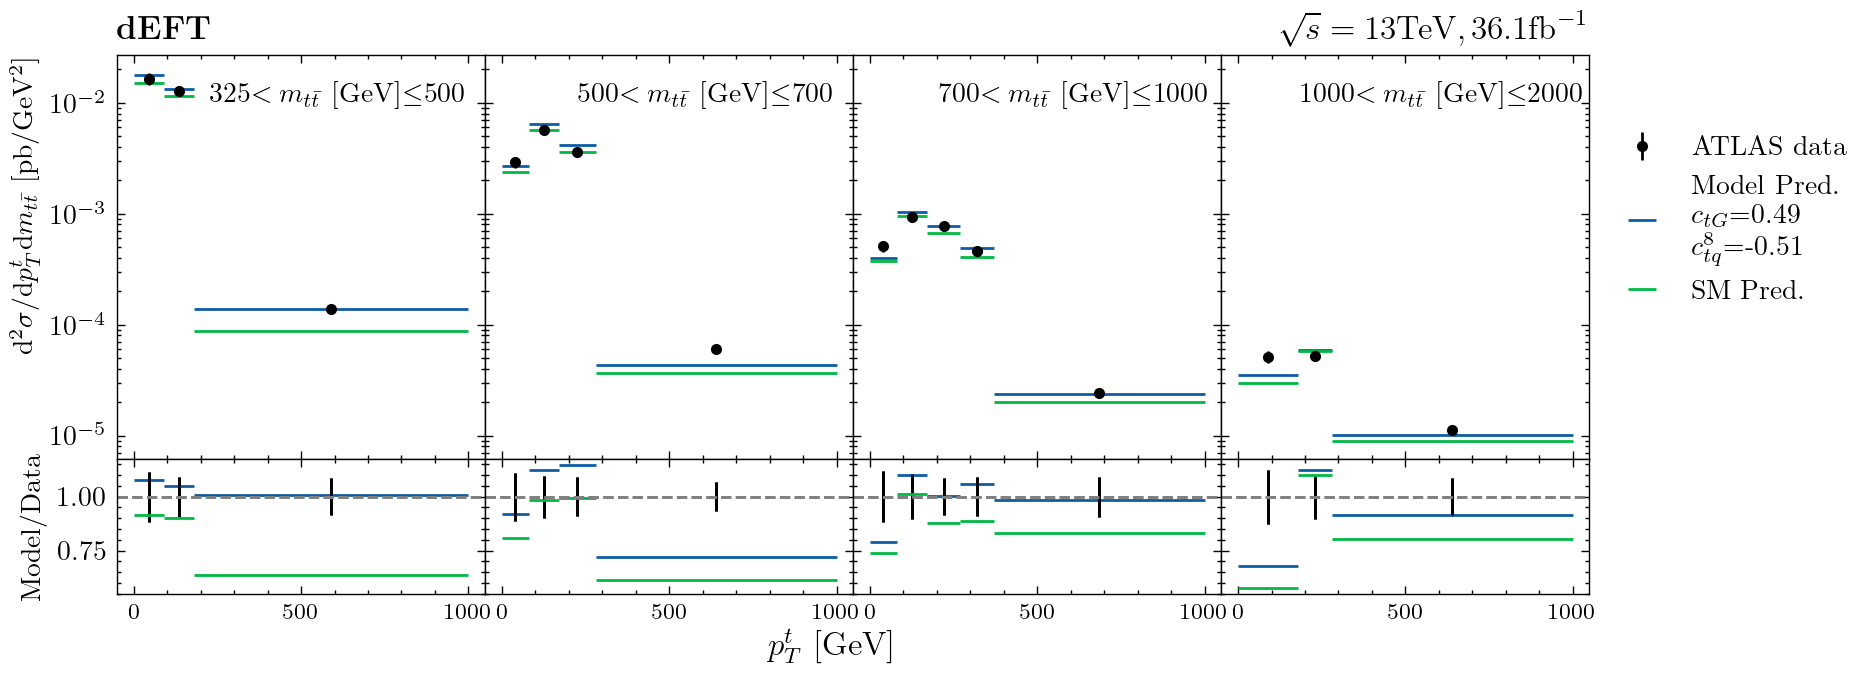
\includegraphics[width=\textwidth]{plots/ATLAS_model_result_2D_2OP.png}
        \caption{2-Dimensional Observable}
        \label{fig:model_result_2D_2OP}
    \end{subfigure}
    \centering
    \caption{Comparison of differential cross section of $t\bar{t}$ production between various morphing model predictions and ATLAS data. This includes model predictions for the optimised Wilson coefficients and for the all zero coefficient case (labelled as SM pred.). The ratio between each model prediction and the data is shown underneath. The errors shown represent statistical and systematic uncertainties of the data.}
    \label{fig:model_result_2OP}
\end{figure}

\section{Conclusion}
\begin{itemize}
    \item describe the analyses done
    \item compare the results briefly
    \item mention the increased constraints on $C_{tg}$
    \item difficulties in measuring $C_{tq}^{8}$
    \item describe future work
    \begin{itemize}
        \item performing at NLO
        \item considering more 4 fermion operators
        \item look at $p_{T}^{t}$ distribution
    \end{itemize}
\end{itemize}

\clearpage
\begingroup
\raggedright{}
\sloppy
\printbibliography{}
\endgroup

\end{document}
